\subsection{What Constitutes Reception?}
\begin{frame}[t]{What Constitutes Reception?}
\small
\begin{block}{}
\textsl{Reception} happens when one planet (A) is in the domicile or exaltation of another planet (B) whom it aspects or conjuncts. The aspect (or conjunction) from planet \textsl{A} must \textsl{perfect} (become exact)  before planet \textsl{B} moves into another sign or a third planet (C) intercedes by completing its own aspect or conjunction with planet \textsl{B}.
\end{block}

\vspace{0.1cm}
\begin{columns}[T, onlytextwidth]
\column{0.5\textwidth}
\Mars\ 10 \Aries\ $\Rightarrow$ \Conjunction\ \Saturn\ 15 \Aries \\
\ul
\vspace{0.2cm}
\Mars\ is applying to \Conjunction\ \Saturn\ who is in \Mars's domicile (\Aries), therefore\\
\Mars\ \textsl{receives} \Saturn\ by domicile, but, \\
\Saturn\ does not receive \Mars\ as he is not in a domicile (\Capricorn, \Aquarius) or Exaltation (\Libra) of \Saturn \\
still, \Mars\ commits his disposition to \Saturn \\
\vspace{0.2cm}
ibn Ezra calls this \textsl{conferring of nature}, Abu Ma'shar, \textsl{pushing nature}; assume it can be likened to an absent host asking a guest to carry out one the host's obligations (this is a weaker form of reception than if \Saturn\ received \Mars)

\column{0.5\textwidth}
\vspace{-0.5cm}
\begin{center}
{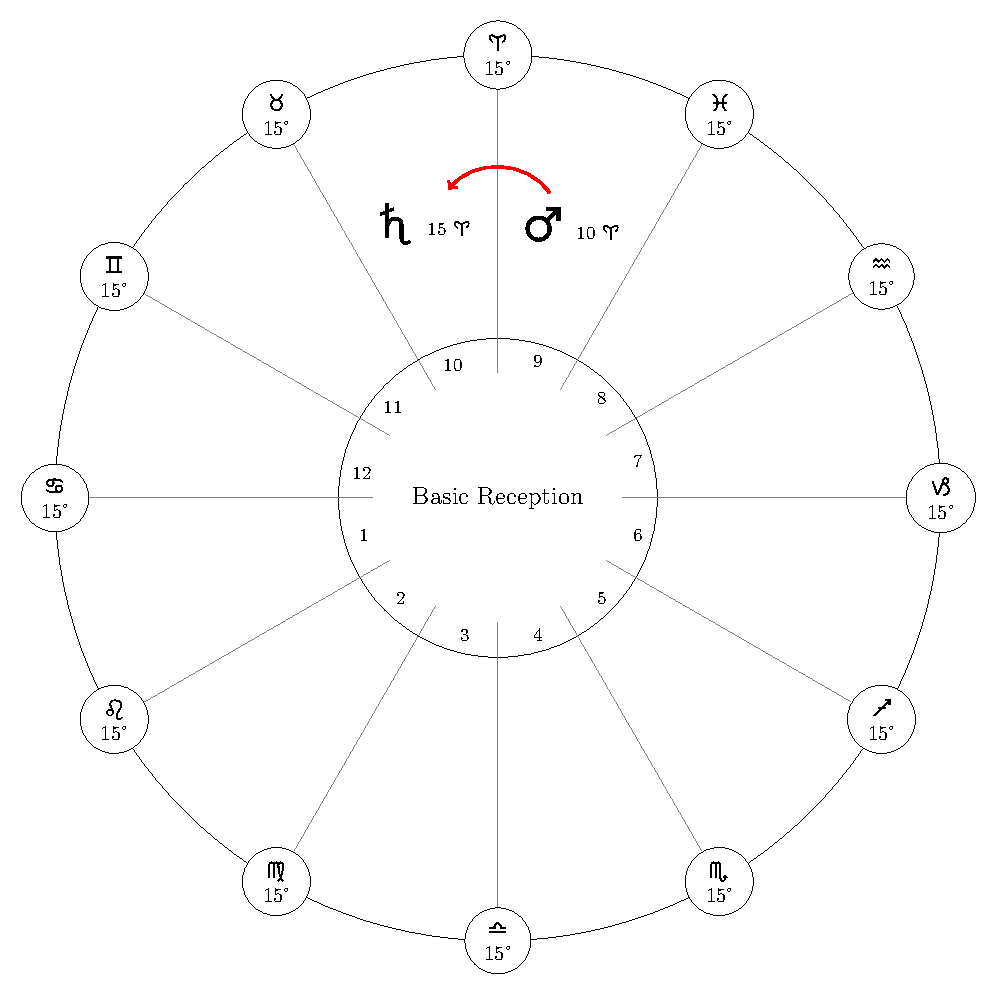
\includegraphics[width=0.9\textwidth]{charts/01-A-receives}} \\
\end{center}

\end{columns}
\vspace{0.2cm}
\end{frame}
% ----------------------------------------------------
\begin{frame}[t]{What Constitutes Reception Continued}
\begin{columns}[T, onlytextwidth]
\column{0.5\textwidth}
\Mars\ 10 \Capricorn\ $\Rightarrow$ \Square\ \Saturn\ 20 \Aries \\
\ul
\vspace{0.5cm}
\Mars\ is in \Saturn's domicile (\Capricorn) applying to \Square\ \Saturn \\
\Saturn\ is in \Mars's domicile (\Aries), therefore, \\
\Mars\ receives \Saturn\ by domicile, and \\
\Saturn\ receives \Mars\ by domicile \\
\vspace{0.25cm}
giving  \textbf{Mutual Reception} [MR] by \textsl{domicile} \\
so \Mars\ receives \Saturn\ and commits his disposition to him and \Saturn\ receives it \\
\vspace{0.25cm}
This is the strongest form of reception

\column{0.5\textwidth}

\begin{center}
{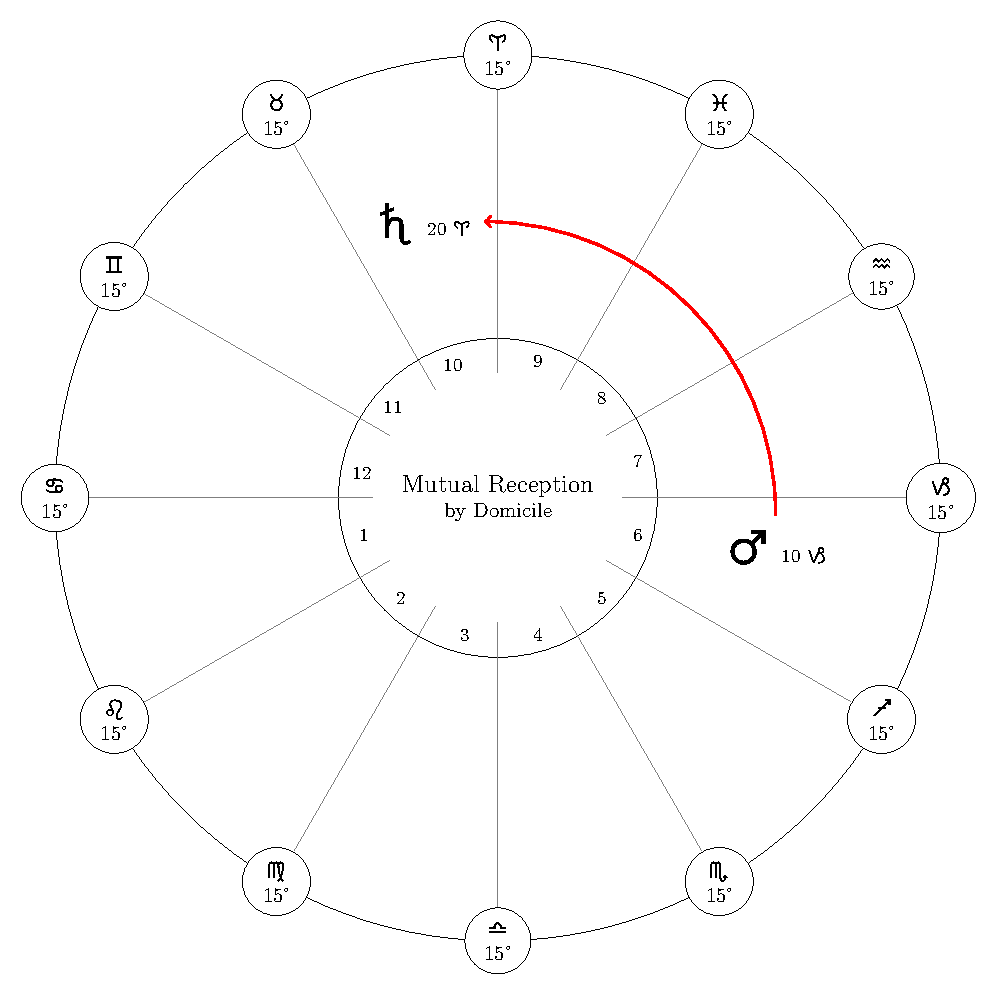
\includegraphics[width=0.9\textwidth]{charts/01-MR-by-domicile}} \\
\end{center}

\end{columns}
\end{frame}
% ----------------------------------------------------
\begin{frame}[t]{What Constitutes Reception Continued}

MR can also happen by Exaltation if the two planets are in each other's signs of exaltation. Masha'allah tells us that if the matter being analyzed has to do with a King, the Exaltation rulers will have more authority over the matter than the domicile rulers. This is considered to be the second strongest form of  reception.

As a general rule, reception is stronger if the planet applied to (usually the heavier planet) receives the applying planet (usually the lighter planet).

Later authors also considered reception by triplicity, term, and face but only considered it to be an \textsl{effective} reception if it involved at least two of these minor dignities i.e. received by triplicity and term or triplicity and face or term and face. Masha'allah does mention these minor dignities in his \textsl{Book of Thoughts and Intentions} but only in relation to determining which planet is stronger than another; he does not use them in any of his reception examples.

\end{frame}